\documentclass[a4paper,12pt,fleqn]{article}		

%%%%%%%%%%%%%%%%%%%%%%%
% Contenu du preambule
%%%%%%%%%%%%%%%%%%%%%%%


\usepackage[left=1.3cm,right=1.3cm,top=1cm,bottom=1.5cm]{geometry}
\usepackage[utf8]{inputenc}		        % Accents, encodage utf8
\usepackage[T1]{fontenc}		        % Encodage des caractères
\usepackage{lmodern}			        % Choix de la fonte (Latin Modern de D. Knuth)
\usepackage[french]{babel}	        	% Les règles de typo. françaises
\usepackage[autolanguage]{numprint}		% Ecrire les nombres correctement \nombre{12354}
%\usepackage{pythontex}
\usepackage{scratch}
\usepackage{multicol} 					% Multi-colonnes
\usepackage{calc} 						% Calculs 
\usepackage{enumerate}					% Pour modifier les numérotations
\usepackage{enumitem}
\usepackage{graphicx}					% Pour insérer des images
\usepackage{tabularx}					% Pour faire des tableaux
\usepackage{pstricks}
\usepackage{pstricks-add}
\usepackage{pst-eucl, pst-plot, pst-fun} 		% figures géométriques
\usepackage{wrapfig}
\usepackage{pgf,tikz,pgfplots}			% Pour les images et figures géométriques
\pgfplotsset{compat=1.15}
\usetikzlibrary{arrows,calc,fit,patterns,plotmarks,shapes.geometric,shapes.misc,shapes.symbols,shapes.arrows,shapes.callouts, shapes.multipart, shapes.gates.logic.US,shapes.gates.logic.IEC, er, automata,backgrounds,chains,topaths,trees,petri,mindmap,matrix, calendar,folding,fadings,through,positioning,scopes,decorations.fractals,decorations.shapes,decorations.text,decorations.pathmorphing,decorations.pathreplacing,decorations.footprints,decorations.markings,shadows,babel} % Charge toutes les librairies de Tikz
%\usetikzlibrary{arrows}
\usepackage{tkz-tab, tkz-fct, tkz-euclide}	% Géométrie euclidienne avec TikZ
%\usetkzobj{all}
\usepackage{amsmath,amsfonts,amssymb,mathrsfs}  % Spécial math
%\usepackage[squaren]{SIunits}			% Pour les unités (gère le conflits avec  \square de l'extension amssymb)
\usepackage{pifont}						% Pour les symboles "ding"
\usepackage{cancel}						% Pour pouvoir barrer les nombres
\usepackage{url} 			        	% Pour afficher correctement les url
\urlstyle{sf}                          	% qui s'afficheront en police sans serif
\usepackage{eurosym}					% Pour utiliser la commande \euro
\usepackage{fancyhdr,lastpage}         	% En-têtes et pieds
	\pagestyle{fancy}                   % de pages personnalisés
\usepackage{fancybox}					% Pour les encadrés
\usepackage{xlop}						% Pour les calculs posés
%\usepackage{standalone}				% Pour avoir un apercu d'un fichier qui sera utilisé avec un input
\usepackage{multido}					% Pour faire des boucles
\usepackage{hyperref}					% Pour gérer les liens hyper-texte
\usepackage{fourier}
%\usepackage{colortbl} 					% Pour des tableaux en couleur
\usepackage{setspace}					% Pour \begin{spacing}{2.0} \end{spacing}
\usepackage{multirow}					% Pour des cellules multilignes dans un tableau

%Mes réglages
			
\setlength{\parindent}{0mm}								% Pas de retrait en début de paragraphe
\renewcommand{\arraystretch}{1.2}						% Interligne dans les tableaux
\renewcommand{\labelenumi}{\textbf{\theenumi{})}}			% Numérotation en gras
\renewcommand{\labelenumii}{\textbf{\theenumii{})}}		% Numérotation de niveau 2 en gras
\renewcommand{\thesection}{\Roman{section}.}				% Numérotation des sections en chiffres romains
\renewcommand{\thesubsection}{\alph{subsection})}			% Numérotation des sous-sections en lettres
\setlength{\columnsep}{40pt}							% largeur pour séparer les colonnes multicols

%Mes macros

\newcounter{exo}          				% déclaration du numéro d'exo (pas utilisé ici)
\setcounter{exo}{0}   					% initialisation du numero
\newcommand{\exo}{					% \exo
  	\stepcounter{exo}        			% incrémentation du numéro
  	\subsection*{Exercice \no{}\theexo}}
  	
\newcommand{\titreitem}[1]{
\Ovalbox{\makebox[.99\linewidth][l]{{Compétence : {#1} }}}
\vspace{0.3cm}} % Titre des items

%%%%%%%%

\pagestyle{empty} 


%%%%%%%%%%%%%%%%%%%%%%%%%%%%%%
% Fin premabule
%%%%%%%%%%%%%%%%%%%%%%%%%%%%%%
\begin{document}
%%%%%%%%%%%%%%%%%%%%%%%%%%%%%%%%%%%%%%%%
%%%%%%%%%%%%%%%%%%%%%%%%%%%%%%%%%%%%%%%%
\setcounter{exo}{0}

%%%%%%%%%%%%%%%%%%%%%%%%%%%%%%%%%%%%%%%%
%  entête du sujet
%%%%%%%%%%%%%%%%%%%%%%%%%%%%%%%%%%%%%%%%

Collège Coat Mez de Daoulas  \hfill  le 22/01/2023

Classe : 6e A \hfill Pierre DETAILLE

\begin{center}
\begin{LARGE} Évaluation de mathématiques \end{LARGE}
\end{center}

%\vspace*{1.5cm}




%%%%%%%%%%%%%%%%%%%%%%%%%%%%%%%%%%%%%%%
% Tableau des compétences (début)
%%%%%%%%%%%%%%%%%%%%%%%%%%%%%%%%%%%%%%%
\begin{footnotesize}

\begin{center}

\begin{tabular}{|p{120mm}|p{8mm}|p{10mm}|p{8mm}|p{8mm}|p{8mm}|}

\hline
\textbf{Compétences évaluées} & \textbf{Rouge} & \textbf{Orange} & \textbf{Bleu} & \textbf{Vert} & \textbf{Autre} \\
\hline


\documentclass[a4paper,12pt,fleqn]{article}		

%%%%%%%%%%%%%%%%%%%%%%%
% Contenu du preambule
%%%%%%%%%%%%%%%%%%%%%%%


\usepackage[left=1.3cm,right=1.3cm,top=1cm,bottom=1.5cm]{geometry}
\usepackage[utf8]{inputenc}		        % Accents, encodage utf8
\usepackage[T1]{fontenc}		        % Encodage des caractères
\usepackage{lmodern}			        % Choix de la fonte (Latin Modern de D. Knuth)
\usepackage[french]{babel}	        	% Les règles de typo. françaises
\usepackage[autolanguage]{numprint}		% Ecrire les nombres correctement \nombre{12354}
%\usepackage{pythontex}
\usepackage{scratch}
\usepackage{multicol} 					% Multi-colonnes
\usepackage{calc} 						% Calculs 
\usepackage{enumerate}					% Pour modifier les numérotations
\usepackage{enumitem}
\usepackage{graphicx}					% Pour insérer des images
\usepackage{tabularx}					% Pour faire des tableaux
\usepackage{pstricks}
\usepackage{pstricks-add}
\usepackage{pst-eucl, pst-plot, pst-fun} 		% figures géométriques
\usepackage{wrapfig}
\usepackage{pgf,tikz,pgfplots}			% Pour les images et figures géométriques
\pgfplotsset{compat=1.15}
\usetikzlibrary{arrows,calc,fit,patterns,plotmarks,shapes.geometric,shapes.misc,shapes.symbols,shapes.arrows,shapes.callouts, shapes.multipart, shapes.gates.logic.US,shapes.gates.logic.IEC, er, automata,backgrounds,chains,topaths,trees,petri,mindmap,matrix, calendar,folding,fadings,through,positioning,scopes,decorations.fractals,decorations.shapes,decorations.text,decorations.pathmorphing,decorations.pathreplacing,decorations.footprints,decorations.markings,shadows,babel} % Charge toutes les librairies de Tikz
%\usetikzlibrary{arrows}
\usepackage{tkz-tab, tkz-fct, tkz-euclide}	% Géométrie euclidienne avec TikZ
%\usetkzobj{all}
\usepackage{amsmath,amsfonts,amssymb,mathrsfs}  % Spécial math
%\usepackage[squaren]{SIunits}			% Pour les unités (gère le conflits avec  \square de l'extension amssymb)
\usepackage{pifont}						% Pour les symboles "ding"
\usepackage{cancel}						% Pour pouvoir barrer les nombres
\usepackage{url} 			        	% Pour afficher correctement les url
\urlstyle{sf}                          	% qui s'afficheront en police sans serif
\usepackage{eurosym}					% Pour utiliser la commande \euro
\usepackage{fancyhdr,lastpage}         	% En-têtes et pieds
	\pagestyle{fancy}                   % de pages personnalisés
\usepackage{fancybox}					% Pour les encadrés
\usepackage{xlop}						% Pour les calculs posés
%\usepackage{standalone}				% Pour avoir un apercu d'un fichier qui sera utilisé avec un input
\usepackage{multido}					% Pour faire des boucles
\usepackage{hyperref}					% Pour gérer les liens hyper-texte
\usepackage{fourier}
%\usepackage{colortbl} 					% Pour des tableaux en couleur
\usepackage{setspace}					% Pour \begin{spacing}{2.0} \end{spacing}
\usepackage{multirow}					% Pour des cellules multilignes dans un tableau

%Mes réglages
			
\setlength{\parindent}{0mm}								% Pas de retrait en début de paragraphe
\renewcommand{\arraystretch}{1.2}						% Interligne dans les tableaux
\renewcommand{\labelenumi}{\textbf{\theenumi{})}}			% Numérotation en gras
\renewcommand{\labelenumii}{\textbf{\theenumii{})}}		% Numérotation de niveau 2 en gras
\renewcommand{\thesection}{\Roman{section}.}				% Numérotation des sections en chiffres romains
\renewcommand{\thesubsection}{\alph{subsection})}			% Numérotation des sous-sections en lettres
\setlength{\columnsep}{40pt}							% largeur pour séparer les colonnes multicols

%Mes macros

\newcounter{exo}          				% déclaration du numéro d'exo (pas utilisé ici)
\setcounter{exo}{0}   					% initialisation du numero
\newcommand{\exo}{					% \exo
  	\stepcounter{exo}        			% incrémentation du numéro
  	\subsection*{Exercice \no{}\theexo}}
  	
\newcommand{\titreitem}[1]{
\Ovalbox{\makebox[.99\linewidth][l]{{Compétence : {#1} }}}
\vspace{0.3cm}} % Titre des items

%%%%%%%%

\pagestyle{empty} 


%%%%%%%%%%%%%%%%%%%%%%%%%%%%%%
% Fin premabule
%%%%%%%%%%%%%%%%%%%%%%%%%%%%%%
\begin{document}
%%%%%%%%%%%%%%%%%%%%%%%%%%%%%%%%%%%%%%%%
%%%%%%%%%%%%%%%%%%%%%%%%%%%%%%%%%%%%%%%%
\setcounter{exo}{0}

%%%%%%%%%%%%%%%%%%%%%%%%%%%%%%%%%%%%%%%%
%  entête du sujet
%%%%%%%%%%%%%%%%%%%%%%%%%%%%%%%%%%%%%%%%

Collège Coat Mez de Daoulas  \hfill  le 22/01/2023

Classe : 6e A \hfill Pierre DETAILLE

\begin{center}
\begin{LARGE} Évaluation de mathématiques \end{LARGE}
\end{center}

%\vspace*{1.5cm}




%%%%%%%%%%%%%%%%%%%%%%%%%%%%%%%%%%%%%%%
% Tableau des compétences (début)
%%%%%%%%%%%%%%%%%%%%%%%%%%%%%%%%%%%%%%%
\begin{footnotesize}

\begin{center}

\begin{tabular}{|p{120mm}|p{8mm}|p{10mm}|p{8mm}|p{8mm}|p{8mm}|}

\hline
\textbf{Compétences évaluées} & \textbf{Rouge} & \textbf{Orange} & \textbf{Bleu} & \textbf{Vert} & \textbf{Autre} \\
\hline


\documentclass[a4paper,12pt,fleqn]{article}		

%%%%%%%%%%%%%%%%%%%%%%%
% Contenu du preambule
%%%%%%%%%%%%%%%%%%%%%%%


\usepackage[left=1.3cm,right=1.3cm,top=1cm,bottom=1.5cm]{geometry}
\usepackage[utf8]{inputenc}		        % Accents, encodage utf8
\usepackage[T1]{fontenc}		        % Encodage des caractères
\usepackage{lmodern}			        % Choix de la fonte (Latin Modern de D. Knuth)
\usepackage[french]{babel}	        	% Les règles de typo. françaises
\usepackage[autolanguage]{numprint}		% Ecrire les nombres correctement \nombre{12354}
%\usepackage{pythontex}
\usepackage{scratch}
\usepackage{multicol} 					% Multi-colonnes
\usepackage{calc} 						% Calculs 
\usepackage{enumerate}					% Pour modifier les numérotations
\usepackage{enumitem}
\usepackage{graphicx}					% Pour insérer des images
\usepackage{tabularx}					% Pour faire des tableaux
\usepackage{pstricks}
\usepackage{pstricks-add}
\usepackage{pst-eucl, pst-plot, pst-fun} 		% figures géométriques
\usepackage{wrapfig}
\usepackage{pgf,tikz,pgfplots}			% Pour les images et figures géométriques
\pgfplotsset{compat=1.15}
\usetikzlibrary{arrows,calc,fit,patterns,plotmarks,shapes.geometric,shapes.misc,shapes.symbols,shapes.arrows,shapes.callouts, shapes.multipart, shapes.gates.logic.US,shapes.gates.logic.IEC, er, automata,backgrounds,chains,topaths,trees,petri,mindmap,matrix, calendar,folding,fadings,through,positioning,scopes,decorations.fractals,decorations.shapes,decorations.text,decorations.pathmorphing,decorations.pathreplacing,decorations.footprints,decorations.markings,shadows,babel} % Charge toutes les librairies de Tikz
%\usetikzlibrary{arrows}
\usepackage{tkz-tab, tkz-fct, tkz-euclide}	% Géométrie euclidienne avec TikZ
%\usetkzobj{all}
\usepackage{amsmath,amsfonts,amssymb,mathrsfs}  % Spécial math
%\usepackage[squaren]{SIunits}			% Pour les unités (gère le conflits avec  \square de l'extension amssymb)
\usepackage{pifont}						% Pour les symboles "ding"
\usepackage{cancel}						% Pour pouvoir barrer les nombres
\usepackage{url} 			        	% Pour afficher correctement les url
\urlstyle{sf}                          	% qui s'afficheront en police sans serif
\usepackage{eurosym}					% Pour utiliser la commande \euro
\usepackage{fancyhdr,lastpage}         	% En-têtes et pieds
	\pagestyle{fancy}                   % de pages personnalisés
\usepackage{fancybox}					% Pour les encadrés
\usepackage{xlop}						% Pour les calculs posés
%\usepackage{standalone}				% Pour avoir un apercu d'un fichier qui sera utilisé avec un input
\usepackage{multido}					% Pour faire des boucles
\usepackage{hyperref}					% Pour gérer les liens hyper-texte
\usepackage{fourier}
%\usepackage{colortbl} 					% Pour des tableaux en couleur
\usepackage{setspace}					% Pour \begin{spacing}{2.0} \end{spacing}
\usepackage{multirow}					% Pour des cellules multilignes dans un tableau

%Mes réglages
			
\setlength{\parindent}{0mm}								% Pas de retrait en début de paragraphe
\renewcommand{\arraystretch}{1.2}						% Interligne dans les tableaux
\renewcommand{\labelenumi}{\textbf{\theenumi{})}}			% Numérotation en gras
\renewcommand{\labelenumii}{\textbf{\theenumii{})}}		% Numérotation de niveau 2 en gras
\renewcommand{\thesection}{\Roman{section}.}				% Numérotation des sections en chiffres romains
\renewcommand{\thesubsection}{\alph{subsection})}			% Numérotation des sous-sections en lettres
\setlength{\columnsep}{40pt}							% largeur pour séparer les colonnes multicols

%Mes macros

\newcounter{exo}          				% déclaration du numéro d'exo (pas utilisé ici)
\setcounter{exo}{0}   					% initialisation du numero
\newcommand{\exo}{					% \exo
  	\stepcounter{exo}        			% incrémentation du numéro
  	\subsection*{Exercice \no{}\theexo}}
  	
\newcommand{\titreitem}[1]{
\Ovalbox{\makebox[.99\linewidth][l]{{Compétence : {#1} }}}
\vspace{0.3cm}} % Titre des items

%%%%%%%%

\pagestyle{empty} 


%%%%%%%%%%%%%%%%%%%%%%%%%%%%%%
% Fin premabule
%%%%%%%%%%%%%%%%%%%%%%%%%%%%%%
\begin{document}
%%%%%%%%%%%%%%%%%%%%%%%%%%%%%%%%%%%%%%%%
%%%%%%%%%%%%%%%%%%%%%%%%%%%%%%%%%%%%%%%%
\setcounter{exo}{0}

%%%%%%%%%%%%%%%%%%%%%%%%%%%%%%%%%%%%%%%%
%  entête du sujet
%%%%%%%%%%%%%%%%%%%%%%%%%%%%%%%%%%%%%%%%

Collège Coat Mez de Daoulas  \hfill  le 22/01/2023

Classe : 6e A \hfill Pierre DETAILLE

\begin{center}
\begin{LARGE} Évaluation de mathématiques \end{LARGE}
\end{center}

%\vspace*{1.5cm}




%%%%%%%%%%%%%%%%%%%%%%%%%%%%%%%%%%%%%%%
% Tableau des compétences (début)
%%%%%%%%%%%%%%%%%%%%%%%%%%%%%%%%%%%%%%%
\begin{footnotesize}

\begin{center}

\begin{tabular}{|p{120mm}|p{8mm}|p{10mm}|p{8mm}|p{8mm}|p{8mm}|}

\hline
\textbf{Compétences évaluées} & \textbf{Rouge} & \textbf{Orange} & \textbf{Bleu} & \textbf{Vert} & \textbf{Autre} \\
\hline


\documentclass[a4paper,12pt,fleqn]{article}		

%%%%%%%%%%%%%%%%%%%%%%%
% Contenu du preambule
%%%%%%%%%%%%%%%%%%%%%%%


\usepackage[left=1.3cm,right=1.3cm,top=1cm,bottom=1.5cm]{geometry}
\usepackage[utf8]{inputenc}		        % Accents, encodage utf8
\usepackage[T1]{fontenc}		        % Encodage des caractères
\usepackage{lmodern}			        % Choix de la fonte (Latin Modern de D. Knuth)
\usepackage[french]{babel}	        	% Les règles de typo. françaises
\usepackage[autolanguage]{numprint}		% Ecrire les nombres correctement \nombre{12354}
%\usepackage{pythontex}
\usepackage{scratch}
\usepackage{multicol} 					% Multi-colonnes
\usepackage{calc} 						% Calculs 
\usepackage{enumerate}					% Pour modifier les numérotations
\usepackage{enumitem}
\usepackage{graphicx}					% Pour insérer des images
\usepackage{tabularx}					% Pour faire des tableaux
\usepackage{pstricks}
\usepackage{pstricks-add}
\usepackage{pst-eucl, pst-plot, pst-fun} 		% figures géométriques
\usepackage{wrapfig}
\usepackage{pgf,tikz,pgfplots}			% Pour les images et figures géométriques
\pgfplotsset{compat=1.15}
\usetikzlibrary{arrows,calc,fit,patterns,plotmarks,shapes.geometric,shapes.misc,shapes.symbols,shapes.arrows,shapes.callouts, shapes.multipart, shapes.gates.logic.US,shapes.gates.logic.IEC, er, automata,backgrounds,chains,topaths,trees,petri,mindmap,matrix, calendar,folding,fadings,through,positioning,scopes,decorations.fractals,decorations.shapes,decorations.text,decorations.pathmorphing,decorations.pathreplacing,decorations.footprints,decorations.markings,shadows,babel} % Charge toutes les librairies de Tikz
%\usetikzlibrary{arrows}
\usepackage{tkz-tab, tkz-fct, tkz-euclide}	% Géométrie euclidienne avec TikZ
%\usetkzobj{all}
\usepackage{amsmath,amsfonts,amssymb,mathrsfs}  % Spécial math
%\usepackage[squaren]{SIunits}			% Pour les unités (gère le conflits avec  \square de l'extension amssymb)
\usepackage{pifont}						% Pour les symboles "ding"
\usepackage{cancel}						% Pour pouvoir barrer les nombres
\usepackage{url} 			        	% Pour afficher correctement les url
\urlstyle{sf}                          	% qui s'afficheront en police sans serif
\usepackage{eurosym}					% Pour utiliser la commande \euro
\usepackage{fancyhdr,lastpage}         	% En-têtes et pieds
	\pagestyle{fancy}                   % de pages personnalisés
\usepackage{fancybox}					% Pour les encadrés
\usepackage{xlop}						% Pour les calculs posés
%\usepackage{standalone}				% Pour avoir un apercu d'un fichier qui sera utilisé avec un input
\usepackage{multido}					% Pour faire des boucles
\usepackage{hyperref}					% Pour gérer les liens hyper-texte
\usepackage{fourier}
%\usepackage{colortbl} 					% Pour des tableaux en couleur
\usepackage{setspace}					% Pour \begin{spacing}{2.0} \end{spacing}
\usepackage{multirow}					% Pour des cellules multilignes dans un tableau

%Mes réglages
			
\setlength{\parindent}{0mm}								% Pas de retrait en début de paragraphe
\renewcommand{\arraystretch}{1.2}						% Interligne dans les tableaux
\renewcommand{\labelenumi}{\textbf{\theenumi{})}}			% Numérotation en gras
\renewcommand{\labelenumii}{\textbf{\theenumii{})}}		% Numérotation de niveau 2 en gras
\renewcommand{\thesection}{\Roman{section}.}				% Numérotation des sections en chiffres romains
\renewcommand{\thesubsection}{\alph{subsection})}			% Numérotation des sous-sections en lettres
\setlength{\columnsep}{40pt}							% largeur pour séparer les colonnes multicols

%Mes macros

\newcounter{exo}          				% déclaration du numéro d'exo (pas utilisé ici)
\setcounter{exo}{0}   					% initialisation du numero
\newcommand{\exo}{					% \exo
  	\stepcounter{exo}        			% incrémentation du numéro
  	\subsection*{Exercice \no{}\theexo}}
  	
\newcommand{\titreitem}[1]{
\Ovalbox{\makebox[.99\linewidth][l]{{Compétence : {#1} }}}
\vspace{0.3cm}} % Titre des items

%%%%%%%%

\pagestyle{empty} 


%%%%%%%%%%%%%%%%%%%%%%%%%%%%%%
% Fin premabule
%%%%%%%%%%%%%%%%%%%%%%%%%%%%%%
\begin{document}
%%%%%%%%%%%%%%%%%%%%%%%%%%%%%%%%%%%%%%%%
%%%%%%%%%%%%%%%%%%%%%%%%%%%%%%%%%%%%%%%%
\setcounter{exo}{0}

%%%%%%%%%%%%%%%%%%%%%%%%%%%%%%%%%%%%%%%%
%  entête du sujet
%%%%%%%%%%%%%%%%%%%%%%%%%%%%%%%%%%%%%%%%

Collège Coat Mez de Daoulas  \hfill  le 22/01/2023

Classe : 6e A \hfill Pierre DETAILLE

\begin{center}
\begin{LARGE} Évaluation de mathématiques \end{LARGE}
\end{center}

%\vspace*{1.5cm}




%%%%%%%%%%%%%%%%%%%%%%%%%%%%%%%%%%%%%%%
% Tableau des compétences (début)
%%%%%%%%%%%%%%%%%%%%%%%%%%%%%%%%%%%%%%%
\begin{footnotesize}

\begin{center}

\begin{tabular}{|p{120mm}|p{8mm}|p{10mm}|p{8mm}|p{8mm}|p{8mm}|}

\hline
\textbf{Compétences évaluées} & \textbf{Rouge} & \textbf{Orange} & \textbf{Bleu} & \textbf{Vert} & \textbf{Autre} \\
\hline


\documentclass[a4paper,12pt,fleqn]{article}		

%%%%%%%%%%%%%%%%%%%%%%%
% Contenu du preambule
%%%%%%%%%%%%%%%%%%%%%%%


\usepackage[left=1.3cm,right=1.3cm,top=1cm,bottom=1.5cm]{geometry}
\usepackage[utf8]{inputenc}		        % Accents, encodage utf8
\usepackage[T1]{fontenc}		        % Encodage des caractères
\usepackage{lmodern}			        % Choix de la fonte (Latin Modern de D. Knuth)
\usepackage[french]{babel}	        	% Les règles de typo. françaises
\usepackage[autolanguage]{numprint}		% Ecrire les nombres correctement \nombre{12354}
%\usepackage{pythontex}
\usepackage{scratch}
\usepackage{multicol} 					% Multi-colonnes
\usepackage{calc} 						% Calculs 
\usepackage{enumerate}					% Pour modifier les numérotations
\usepackage{enumitem}
\usepackage{graphicx}					% Pour insérer des images
\usepackage{tabularx}					% Pour faire des tableaux
\usepackage{pstricks}
\usepackage{pstricks-add}
\usepackage{pst-eucl, pst-plot, pst-fun} 		% figures géométriques
\usepackage{wrapfig}
\usepackage{pgf,tikz,pgfplots}			% Pour les images et figures géométriques
\pgfplotsset{compat=1.15}
\usetikzlibrary{arrows,calc,fit,patterns,plotmarks,shapes.geometric,shapes.misc,shapes.symbols,shapes.arrows,shapes.callouts, shapes.multipart, shapes.gates.logic.US,shapes.gates.logic.IEC, er, automata,backgrounds,chains,topaths,trees,petri,mindmap,matrix, calendar,folding,fadings,through,positioning,scopes,decorations.fractals,decorations.shapes,decorations.text,decorations.pathmorphing,decorations.pathreplacing,decorations.footprints,decorations.markings,shadows,babel} % Charge toutes les librairies de Tikz
%\usetikzlibrary{arrows}
\usepackage{tkz-tab, tkz-fct, tkz-euclide}	% Géométrie euclidienne avec TikZ
%\usetkzobj{all}
\usepackage{amsmath,amsfonts,amssymb,mathrsfs}  % Spécial math
%\usepackage[squaren]{SIunits}			% Pour les unités (gère le conflits avec  \square de l'extension amssymb)
\usepackage{pifont}						% Pour les symboles "ding"
\usepackage{cancel}						% Pour pouvoir barrer les nombres
\usepackage{url} 			        	% Pour afficher correctement les url
\urlstyle{sf}                          	% qui s'afficheront en police sans serif
\usepackage{eurosym}					% Pour utiliser la commande \euro
\usepackage{fancyhdr,lastpage}         	% En-têtes et pieds
	\pagestyle{fancy}                   % de pages personnalisés
\usepackage{fancybox}					% Pour les encadrés
\usepackage{xlop}						% Pour les calculs posés
%\usepackage{standalone}				% Pour avoir un apercu d'un fichier qui sera utilisé avec un input
\usepackage{multido}					% Pour faire des boucles
\usepackage{hyperref}					% Pour gérer les liens hyper-texte
\usepackage{fourier}
%\usepackage{colortbl} 					% Pour des tableaux en couleur
\usepackage{setspace}					% Pour \begin{spacing}{2.0} \end{spacing}
\usepackage{multirow}					% Pour des cellules multilignes dans un tableau

%Mes réglages
			
\setlength{\parindent}{0mm}								% Pas de retrait en début de paragraphe
\renewcommand{\arraystretch}{1.2}						% Interligne dans les tableaux
\renewcommand{\labelenumi}{\textbf{\theenumi{})}}			% Numérotation en gras
\renewcommand{\labelenumii}{\textbf{\theenumii{})}}		% Numérotation de niveau 2 en gras
\renewcommand{\thesection}{\Roman{section}.}				% Numérotation des sections en chiffres romains
\renewcommand{\thesubsection}{\alph{subsection})}			% Numérotation des sous-sections en lettres
\setlength{\columnsep}{40pt}							% largeur pour séparer les colonnes multicols

%Mes macros

\newcounter{exo}          				% déclaration du numéro d'exo (pas utilisé ici)
\setcounter{exo}{0}   					% initialisation du numero
\newcommand{\exo}{					% \exo
  	\stepcounter{exo}        			% incrémentation du numéro
  	\subsection*{Exercice \no{}\theexo}}
  	
\newcommand{\titreitem}[1]{
\Ovalbox{\makebox[.99\linewidth][l]{{Compétence : {#1} }}}
\vspace{0.3cm}} % Titre des items

%%%%%%%%

\pagestyle{empty} 


%%%%%%%%%%%%%%%%%%%%%%%%%%%%%%
% Fin premabule
%%%%%%%%%%%%%%%%%%%%%%%%%%%%%%
\begin{document}
%%%%%%%%%%%%%%%%%%%%%%%%%%%%%%%%%%%%%%%%
%%%%%%%%%%%%%%%%%%%%%%%%%%%%%%%%%%%%%%%%
\setcounter{exo}{0}

%%%%%%%%%%%%%%%%%%%%%%%%%%%%%%%%%%%%%%%%
%  entête du sujet
%%%%%%%%%%%%%%%%%%%%%%%%%%%%%%%%%%%%%%%%

Collège Coat Mez de Daoulas  \hfill  le 22/01/2023

Classe : 6e A \hfill Pierre DETAILLE

\begin{center}
\begin{LARGE} Évaluation de mathématiques \end{LARGE}
\end{center}

%\vspace*{1.5cm}




%%%%%%%%%%%%%%%%%%%%%%%%%%%%%%%%%%%%%%%
% Tableau des compétences (début)
%%%%%%%%%%%%%%%%%%%%%%%%%%%%%%%%%%%%%%%
\begin{footnotesize}

\begin{center}

\begin{tabular}{|p{120mm}|p{8mm}|p{10mm}|p{8mm}|p{8mm}|p{8mm}|}

\hline
\textbf{Compétences évaluées} & \textbf{Rouge} & \textbf{Orange} & \textbf{Bleu} & \textbf{Vert} & \textbf{Autre} \\
\hline


\documentclass[a4paper,12pt,fleqn]{article}		

%%%%%%%%%%%%%%%%%%%%%%%
% Contenu du preambule
%%%%%%%%%%%%%%%%%%%%%%%


\usepackage[left=1.3cm,right=1.3cm,top=1cm,bottom=1.5cm]{geometry}
\usepackage[utf8]{inputenc}		        % Accents, encodage utf8
\usepackage[T1]{fontenc}		        % Encodage des caractères
\usepackage{lmodern}			        % Choix de la fonte (Latin Modern de D. Knuth)
\usepackage[french]{babel}	        	% Les règles de typo. françaises
\usepackage[autolanguage]{numprint}		% Ecrire les nombres correctement \nombre{12354}
%\usepackage{pythontex}
\usepackage{scratch}
\usepackage{multicol} 					% Multi-colonnes
\usepackage{calc} 						% Calculs 
\usepackage{enumerate}					% Pour modifier les numérotations
\usepackage{enumitem}
\usepackage{graphicx}					% Pour insérer des images
\usepackage{tabularx}					% Pour faire des tableaux
\usepackage{pstricks}
\usepackage{pstricks-add}
\usepackage{pst-eucl, pst-plot, pst-fun} 		% figures géométriques
\usepackage{wrapfig}
\usepackage{pgf,tikz,pgfplots}			% Pour les images et figures géométriques
\pgfplotsset{compat=1.15}
\usetikzlibrary{arrows,calc,fit,patterns,plotmarks,shapes.geometric,shapes.misc,shapes.symbols,shapes.arrows,shapes.callouts, shapes.multipart, shapes.gates.logic.US,shapes.gates.logic.IEC, er, automata,backgrounds,chains,topaths,trees,petri,mindmap,matrix, calendar,folding,fadings,through,positioning,scopes,decorations.fractals,decorations.shapes,decorations.text,decorations.pathmorphing,decorations.pathreplacing,decorations.footprints,decorations.markings,shadows,babel} % Charge toutes les librairies de Tikz
%\usetikzlibrary{arrows}
\usepackage{tkz-tab, tkz-fct, tkz-euclide}	% Géométrie euclidienne avec TikZ
%\usetkzobj{all}
\usepackage{amsmath,amsfonts,amssymb,mathrsfs}  % Spécial math
%\usepackage[squaren]{SIunits}			% Pour les unités (gère le conflits avec  \square de l'extension amssymb)
\usepackage{pifont}						% Pour les symboles "ding"
\usepackage{cancel}						% Pour pouvoir barrer les nombres
\usepackage{url} 			        	% Pour afficher correctement les url
\urlstyle{sf}                          	% qui s'afficheront en police sans serif
\usepackage{eurosym}					% Pour utiliser la commande \euro
\usepackage{fancyhdr,lastpage}         	% En-têtes et pieds
	\pagestyle{fancy}                   % de pages personnalisés
\usepackage{fancybox}					% Pour les encadrés
\usepackage{xlop}						% Pour les calculs posés
%\usepackage{standalone}				% Pour avoir un apercu d'un fichier qui sera utilisé avec un input
\usepackage{multido}					% Pour faire des boucles
\usepackage{hyperref}					% Pour gérer les liens hyper-texte
\usepackage{fourier}
%\usepackage{colortbl} 					% Pour des tableaux en couleur
\usepackage{setspace}					% Pour \begin{spacing}{2.0} \end{spacing}
\usepackage{multirow}					% Pour des cellules multilignes dans un tableau

%Mes réglages
			
\setlength{\parindent}{0mm}								% Pas de retrait en début de paragraphe
\renewcommand{\arraystretch}{1.2}						% Interligne dans les tableaux
\renewcommand{\labelenumi}{\textbf{\theenumi{})}}			% Numérotation en gras
\renewcommand{\labelenumii}{\textbf{\theenumii{})}}		% Numérotation de niveau 2 en gras
\renewcommand{\thesection}{\Roman{section}.}				% Numérotation des sections en chiffres romains
\renewcommand{\thesubsection}{\alph{subsection})}			% Numérotation des sous-sections en lettres
\setlength{\columnsep}{40pt}							% largeur pour séparer les colonnes multicols

%Mes macros

\newcounter{exo}          				% déclaration du numéro d'exo (pas utilisé ici)
\setcounter{exo}{0}   					% initialisation du numero
\newcommand{\exo}{					% \exo
  	\stepcounter{exo}        			% incrémentation du numéro
  	\subsection*{Exercice \no{}\theexo}}
  	
\newcommand{\titreitem}[1]{
\Ovalbox{\makebox[.99\linewidth][l]{{Compétence : {#1} }}}
\vspace{0.3cm}} % Titre des items

%%%%%%%%

\pagestyle{empty} 


%%%%%%%%%%%%%%%%%%%%%%%%%%%%%%
% Fin premabule
%%%%%%%%%%%%%%%%%%%%%%%%%%%%%%
\begin{document}
%%%%%%%%%%%%%%%%%%%%%%%%%%%%%%%%%%%%%%%%
%%%%%%%%%%%%%%%%%%%%%%%%%%%%%%%%%%%%%%%%
\setcounter{exo}{0}

%%%%%%%%%%%%%%%%%%%%%%%%%%%%%%%%%%%%%%%%
%  entête du sujet
%%%%%%%%%%%%%%%%%%%%%%%%%%%%%%%%%%%%%%%%

Collège Coat Mez de Daoulas  \hfill  le 22/01/2023

Classe : 6e A \hfill Pierre DETAILLE

\begin{center}
\begin{LARGE} Évaluation de mathématiques \end{LARGE}
\end{center}

%\vspace*{1.5cm}




%%%%%%%%%%%%%%%%%%%%%%%%%%%%%%%%%%%%%%%
% Tableau des compétences (début)
%%%%%%%%%%%%%%%%%%%%%%%%%%%%%%%%%%%%%%%
\begin{footnotesize}

\begin{center}

\begin{tabular}{|p{120mm}|p{8mm}|p{10mm}|p{8mm}|p{8mm}|p{8mm}|}

\hline
\textbf{Compétences évaluées} & \textbf{Rouge} & \textbf{Orange} & \textbf{Bleu} & \textbf{Vert} & \textbf{Autre} \\
\hline


*  Additionner, soustraire des nombres relatifs  & & & & & \\ 
\hline
*  Démontrer : utiliser un raisonnement logique et des règles établies pour parvenir à une conclusion.  & & & & & \\ 
\hline
\end{tabular}
\end{center}
\end{footnotesize}
\begin{minipage}{0.99\linewidth}

\exo

\emph{La calculatrice n'est pas autorisée.}

% \titreitem{Calculer des additions et des soustractions de nombres relatifs.}

Calculer, en indiquant, quand il y en a, les différentes étapes. 

\begin{enumerate}

\begin{multicols}{2}

\item $ (-12)+(+8)= $

\item $ (-15)+(-3)= $

\item $ (+40)-(-15)= $

\item $ (-35)-(+12)= $

\item $ (-20)+(+16)-(+30)+(+20)-(-15) = $

\end{multicols}

\end{enumerate}

\end{minipage}

\vspace{0.5cm}

\medskip
\begin{minipage}{0.99\linewidth}

\exo

\begin{multicols}{2}
Utiliser les informations données sur cette figure à main levée pour démontrer que les triangles $IML$ et $MKL$ sont semblables

\begin{center}

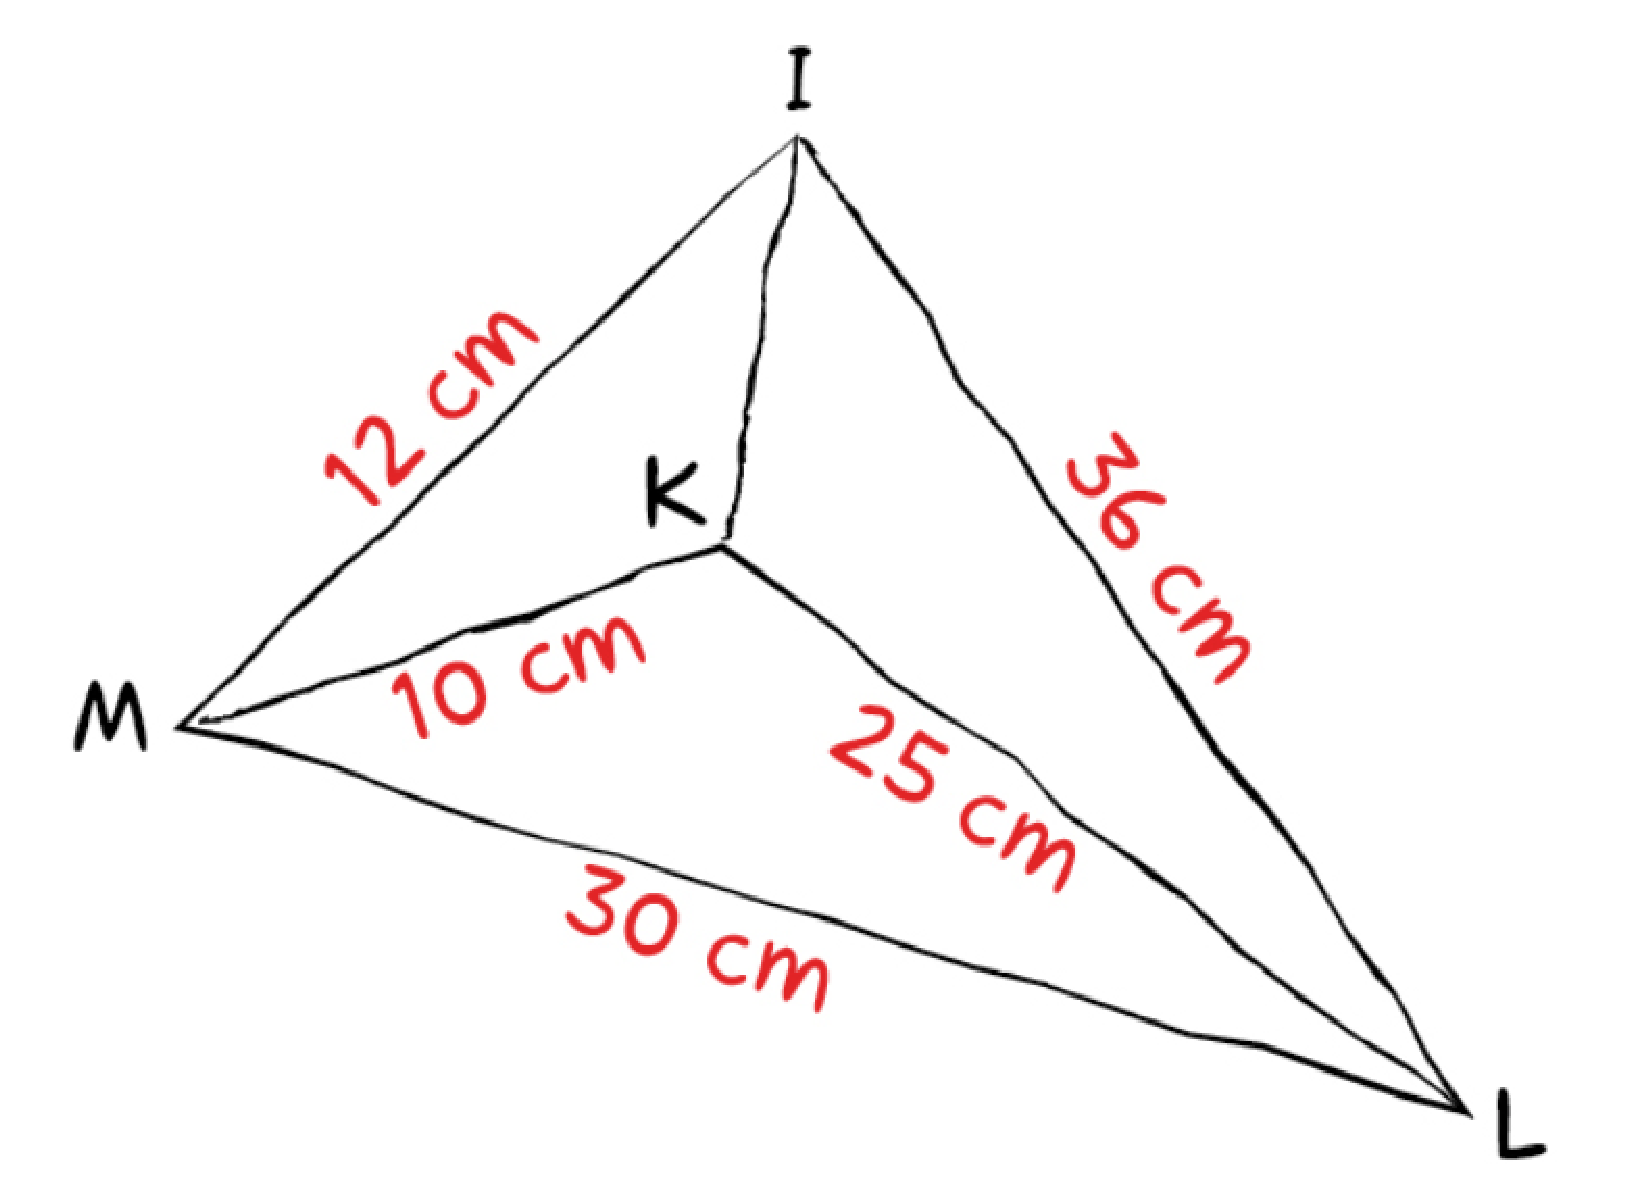
\includegraphics[scale=.18]{items/MathsP4C42.eps}

\end{center}

\end{multicols}

\end{minipage}

\vspace{0.5cm}

\medskip
\newpage
%%%%%%%%%%%%%%%%%%%%%%%%%%%%%%%%%%%%%%%%
%%%%%%%%%%%%%%%%%%%%%%%%%%%%%%%%%%%%%%%%
\setcounter{exo}{0}

%%%%%%%%%%%%%%%%%%%%%%%%%%%%%%%%%%%%%%%%
%  entête du sujet
%%%%%%%%%%%%%%%%%%%%%%%%%%%%%%%%%%%%%%%%

Collège Coat Mez de Daoulas  \hfill  le 22/01/2023

Classe : 6e A \hfill Julie CORNE

\begin{center}
\begin{LARGE} Évaluation de mathématiques \end{LARGE}
\end{center}

%\vspace*{1.5cm}




%%%%%%%%%%%%%%%%%%%%%%%%%%%%%%%%%%%%%%%
% Tableau des compétences (début)
%%%%%%%%%%%%%%%%%%%%%%%%%%%%%%%%%%%%%%%
\begin{footnotesize}

\begin{center}

\begin{tabular}{|p{120mm}|p{8mm}|p{10mm}|p{8mm}|p{8mm}|p{8mm}|}

\hline
\textbf{Compétences évaluées} & \textbf{Rouge} & \textbf{Orange} & \textbf{Bleu} & \textbf{Vert} & \textbf{Autre} \\
\hline


*  Additionner, soustraire des nombres relatifs  & & & & & \\ 
\hline
*  Décomposer un nombre entier en produit de facteurs premiers  & & & & & \\ 
\hline
*  Simplifier une fraction donnée pour la rendre irréductible  & & & & & \\ 
\hline
\end{tabular}
\end{center}
\end{footnotesize}
\begin{minipage}{0.99\linewidth}

\exo

\emph{La calculatrice n'est pas autorisée.}

% \titreitem{Calculer des additions et des soustractions de nombres relatifs.}

Calculer, en indiquant, quand il y en a, les différentes étapes. 

\begin{enumerate}

\begin{multicols}{2}

\item $ (-12)+(+8)= $

\item $ (-15)+(-3)= $

\item $ (+40)-(-15)= $

\item $ (-35)-(+12)= $

\item $ (-20)+(+16)-(+30)+(+20)-(-15) = $

\end{multicols}

\end{enumerate}

\end{minipage}

\vspace{0.5cm}

\medskip
\begin{minipage}{0.99\linewidth}

\exo
%\titreitem{Décomposer un entier en produit de facteurs premiers.}

\begin{enumerate}

\item Décomposer $700$ en produit de facteurs premiers.
\item Décomposer $54$ en produit de facteurs premiers.
\item Décomposer $175$ en produit de facteurs premiers.

\end{enumerate}
\end{minipage}

\vspace{0.5cm}

\medskip
\begin{minipage}{0.99\linewidth}

\exo

Dans cet exercice l'usage de la calculatrice est interdit.

\begin{enumerate}

\item Simplifier et rendre irréductible la fraction $\dfrac{360}{450}$ (méthode libre, mais il faut détailler les calculs).
\item Décomposer $54$ en produit de facteurs premiers.
\item Décomposer $210$ en produit de facteurs premiers.
\item Utiliser les résultats des deux questions précédentes pour rendre irréductible la fraction $\dfrac{54}{210}$
\end{enumerate}
\end{minipage}

\vspace{0.5cm}

\medskip
\newpage
%%%%%%%%%%%%%%%%%%%%%%%%%%%%%%%%%%%%%%%%
%%%%%%%%%%%%%%%%%%%%%%%%%%%%%%%%%%%%%%%%
\setcounter{exo}{0}

%%%%%%%%%%%%%%%%%%%%%%%%%%%%%%%%%%%%%%%%
%  entête du sujet
%%%%%%%%%%%%%%%%%%%%%%%%%%%%%%%%%%%%%%%%

Collège Coat Mez de Daoulas  \hfill  le 22/01/2023

Classe : 6e A \hfill Angèle LANUIT

\begin{center}
\begin{LARGE} Évaluation de mathématiques \end{LARGE}
\end{center}

%\vspace*{1.5cm}




%%%%%%%%%%%%%%%%%%%%%%%%%%%%%%%%%%%%%%%
% Tableau des compétences (début)
%%%%%%%%%%%%%%%%%%%%%%%%%%%%%%%%%%%%%%%
\begin{footnotesize}

\begin{center}

\begin{tabular}{|p{120mm}|p{8mm}|p{10mm}|p{8mm}|p{8mm}|p{8mm}|}

\hline
\textbf{Compétences évaluées} & \textbf{Rouge} & \textbf{Orange} & \textbf{Bleu} & \textbf{Vert} & \textbf{Autre} \\
\hline


*  Connaitre la notion de nombres premiers  & & & & & \\ 
\hline
*  Connaitre et utiliser la notion de diviseur, de multiple  & & & & & \\ 
\hline
\end{tabular}
\end{center}
\end{footnotesize}
\begin{minipage}{0.99\linewidth}

\exo

% \titreitem{Connaitre les nombres premiers.}


\begin{enumerate}

\item Qu'est-ce qu'un nombre premier ?

\item $14 625$ est-il un nombre premier ? Justifier.

\item $31$ est-il un nombre premier ? Justifier.

\item $121$ est-il un nombre premier ? Justifier.

\end{enumerate}

\end{minipage}

\vspace{0.5cm}

\medskip
\begin{minipage}{0.99\linewidth}

\exo

% \titreitem{Connaitre et utiliser les diviseurs et les multiples d'un nombre.}


\begin{enumerate}

\item Écrire tous les diviseurs de $72$ ?

\item Écrire tous les diviseurs de $96$ ?

\item Quel est le plus grand diviseur commun à $72$ et $96$ ? En déduire la fraction irréductible égale à $\dfrac{96}{72}$.

\item Écrire les 7 premiers multiples de 6.

\item Écrire les 7 premiers multiples de 10.

\item Quel est le plus petit multiple commun à 6 et 10 ? 


\end{enumerate}

\end{minipage}

\vspace{0.5cm}

\medskip
\newpage
%%%%%%%%%%%%%%%%%%%%%%%%%%%%%%%%%%%%%%%%
%%%%%%%%%%%%%%%%%%%%%%%%%%%%%%%%%%%%%%%%
\setcounter{exo}{0}

%%%%%%%%%%%%%%%%%%%%%%%%%%%%%%%%%%%%%%%%
%  entête du sujet
%%%%%%%%%%%%%%%%%%%%%%%%%%%%%%%%%%%%%%%%

Collège Coat Mez de Daoulas  \hfill  le 22/01/2023

Classe : 6e A \hfill Léa PATOR

\begin{center}
\begin{LARGE} Évaluation de mathématiques \end{LARGE}
\end{center}

%\vspace*{1.5cm}




%%%%%%%%%%%%%%%%%%%%%%%%%%%%%%%%%%%%%%%
% Tableau des compétences (début)
%%%%%%%%%%%%%%%%%%%%%%%%%%%%%%%%%%%%%%%
\begin{footnotesize}

\begin{center}

\begin{tabular}{|p{120mm}|p{8mm}|p{10mm}|p{8mm}|p{8mm}|p{8mm}|}

\hline
\textbf{Compétences évaluées} & \textbf{Rouge} & \textbf{Orange} & \textbf{Bleu} & \textbf{Vert} & \textbf{Autre} \\
\hline


*  Reconnaître et utiliser des triangles semblables.  & & & & & \\ 
\hline
\end{tabular}
\end{center}
\end{footnotesize}
\begin{minipage}{0.99\linewidth}

\exo

Dans le triangle $BGF$, on sait que $\widehat{FBG}$ mesure $46$\degre et que $\widehat{BGF}$ mesure $103$\degre. On sait aussi que D est un point du segment $[BF]$, que C est un point du segment $[BG]$ et que $\widehat{BDC}$ mesure $31$\degre.

		\begin{enumerate}
		\item Faire un croquis, sur la copie, et y coder les informations données.
		\item Prouver que les triangles $BCD$ et $BFG$ sont semblables.
		\item $BD= 4$~cm, $DC=3$~cm et $BF=6$~cm. Quel est le coefficient d'agrandissement qui permet de passer du triangle $BCD$ au triangle $BFG$ ? (Justifier votre réponse).
		\end{enumerate}	

\end{minipage}

\vspace{0.5cm}
\medskip
\newpage
%%%%%%%%%%%%%%%%%%%%%%%%%%%%%%%%%%%%%%%%
%%%%%%%%%%%%%%%%%%%%%%%%%%%%%%%%%%%%%%%%
\setcounter{exo}{0}

%%%%%%%%%%%%%%%%%%%%%%%%%%%%%%%%%%%%%%%%
%  entête du sujet
%%%%%%%%%%%%%%%%%%%%%%%%%%%%%%%%%%%%%%%%

Collège Coat Mez de Daoulas  \hfill  le 22/01/2023

Classe : 6e A \hfill Jean NAIMAR

\begin{center}
\begin{LARGE} Évaluation de mathématiques \end{LARGE}
\end{center}

%\vspace*{1.5cm}




%%%%%%%%%%%%%%%%%%%%%%%%%%%%%%%%%%%%%%%
% Tableau des compétences (début)
%%%%%%%%%%%%%%%%%%%%%%%%%%%%%%%%%%%%%%%
\begin{footnotesize}

\begin{center}

\begin{tabular}{|p{120mm}|p{8mm}|p{10mm}|p{8mm}|p{8mm}|p{8mm}|}

\hline
\textbf{Compétences évaluées} & \textbf{Rouge} & \textbf{Orange} & \textbf{Bleu} & \textbf{Vert} & \textbf{Autre} \\
\hline


*  Connaitre la notion de nombres premiers  & & & & & \\ 
\hline
*  Décomposer un nombre entier en produit de facteurs premiers  & & & & & \\ 
\hline
*  Simplifier une fraction donnée pour la rendre irréductible  & & & & & \\ 
\hline
\end{tabular}
\end{center}
\end{footnotesize}
\begin{minipage}{0.99\linewidth}

\exo

% \titreitem{Connaitre les nombres premiers.}


\begin{enumerate}

\item Qu'est-ce qu'un nombre premier ?

\item $14 625$ est-il un nombre premier ? Justifier.

\item $31$ est-il un nombre premier ? Justifier.

\item $121$ est-il un nombre premier ? Justifier.

\end{enumerate}

\end{minipage}

\vspace{0.5cm}

\medskip
\begin{minipage}{0.99\linewidth}

\exo
%\titreitem{Décomposer un entier en produit de facteurs premiers.}

\begin{enumerate}

\item Décomposer $700$ en produit de facteurs premiers.
\item Décomposer $54$ en produit de facteurs premiers.
\item Décomposer $175$ en produit de facteurs premiers.

\end{enumerate}
\end{minipage}

\vspace{0.5cm}

\medskip
\begin{minipage}{0.99\linewidth}

\exo

Dans cet exercice l'usage de la calculatrice est interdit.

\begin{enumerate}

\item Simplifier et rendre irréductible la fraction $\dfrac{360}{450}$ (méthode libre, mais il faut détailler les calculs).
\item Décomposer $54$ en produit de facteurs premiers.
\item Décomposer $210$ en produit de facteurs premiers.
\item Utiliser les résultats des deux questions précédentes pour rendre irréductible la fraction $\dfrac{54}{210}$
\end{enumerate}
\end{minipage}

\vspace{0.5cm}

\medskip
\newpage
%%%%%%%%%%%%%%%%%%%%%%%%%%%%%%%%%%%%%%%%
%%%%%%%%%%%%%%%%%%%%%%%%%%%%%%%%%%%%%%%%
\setcounter{exo}{0}

%%%%%%%%%%%%%%%%%%%%%%%%%%%%%%%%%%%%%%%%
%  entête du sujet
%%%%%%%%%%%%%%%%%%%%%%%%%%%%%%%%%%%%%%%%

Collège Coat Mez de Daoulas  \hfill  le 22/01/2023

Classe : 6e A \hfill Patrice QUETOUT

\begin{center}
\begin{LARGE} Évaluation de mathématiques \end{LARGE}
\end{center}

%\vspace*{1.5cm}




%%%%%%%%%%%%%%%%%%%%%%%%%%%%%%%%%%%%%%%
% Tableau des compétences (début)
%%%%%%%%%%%%%%%%%%%%%%%%%%%%%%%%%%%%%%%
\begin{footnotesize}

\begin{center}

\begin{tabular}{|p{120mm}|p{8mm}|p{10mm}|p{8mm}|p{8mm}|p{8mm}|}

\hline
\textbf{Compétences évaluées} & \textbf{Rouge} & \textbf{Orange} & \textbf{Bleu} & \textbf{Vert} & \textbf{Autre} \\
\hline


*  Additionner, soustraire des nombres relatifs  & & & & & \\ 
\hline
*  Reconnaître et utiliser des triangles semblables.  & & & & & \\ 
\hline
\end{tabular}
\end{center}
\end{footnotesize}
\begin{minipage}{0.99\linewidth}

\exo

\emph{La calculatrice n'est pas autorisée.}

% \titreitem{Calculer des additions et des soustractions de nombres relatifs.}

Calculer, en indiquant, quand il y en a, les différentes étapes. 

\begin{enumerate}

\begin{multicols}{2}

\item $ (-12)+(+8)= $

\item $ (-15)+(-3)= $

\item $ (+40)-(-15)= $

\item $ (-35)-(+12)= $

\item $ (-20)+(+16)-(+30)+(+20)-(-15) = $

\end{multicols}

\end{enumerate}

\end{minipage}

\vspace{0.5cm}

\medskip
\begin{minipage}{0.99\linewidth}

\exo

Dans le triangle $BGF$, on sait que $\widehat{FBG}$ mesure $46$\degre et que $\widehat{BGF}$ mesure $103$\degre. On sait aussi que D est un point du segment $[BF]$, que C est un point du segment $[BG]$ et que $\widehat{BDC}$ mesure $31$\degre.

		\begin{enumerate}
		\item Faire un croquis, sur la copie, et y coder les informations données.
		\item Prouver que les triangles $BCD$ et $BFG$ sont semblables.
		\item $BD= 4$~cm, $DC=3$~cm et $BF=6$~cm. Quel est le coefficient d'agrandissement qui permet de passer du triangle $BCD$ au triangle $BFG$ ? (Justifier votre réponse).
		\end{enumerate}	

\end{minipage}

\vspace{0.5cm}
\medskip
\newpage
%%%%%%%%%%%%%%%%%%%%%%%%%%%%%%%%%%%%%%%%
%%%%%%%%%%%%%%%%%%%%%%%%%%%%%%%%%%%%%%%%
\setcounter{exo}{0}

%%%%%%%%%%%%%%%%%%%%%%%%%%%%%%%%%%%%%%%%
%  entête du sujet
%%%%%%%%%%%%%%%%%%%%%%%%%%%%%%%%%%%%%%%%

Collège Coat Mez de Daoulas  \hfill  le 22/01/2023

Classe : 6e A \hfill Cyril DUPONT

\begin{center}
\begin{LARGE} Évaluation de mathématiques \end{LARGE}
\end{center}

%\vspace*{1.5cm}




%%%%%%%%%%%%%%%%%%%%%%%%%%%%%%%%%%%%%%%
% Tableau des compétences (début)
%%%%%%%%%%%%%%%%%%%%%%%%%%%%%%%%%%%%%%%
\begin{footnotesize}

\begin{center}

\begin{tabular}{|p{120mm}|p{8mm}|p{10mm}|p{8mm}|p{8mm}|p{8mm}|}

\hline
\textbf{Compétences évaluées} & \textbf{Rouge} & \textbf{Orange} & \textbf{Bleu} & \textbf{Vert} & \textbf{Autre} \\
\hline


*  Additionner, soustraire des nombres relatifs  & & & & & \\ 
\hline
*  Décomposer un nombre entier en produit de facteurs premiers  & & & & & \\ 
\hline
*  Simplifier une fraction donnée pour la rendre irréductible  & & & & & \\ 
\hline
\end{tabular}
\end{center}
\end{footnotesize}
\begin{minipage}{0.99\linewidth}

\exo

\emph{La calculatrice n'est pas autorisée.}

% \titreitem{Calculer des additions et des soustractions de nombres relatifs.}

Calculer, en indiquant, quand il y en a, les différentes étapes. 

\begin{enumerate}

\begin{multicols}{2}

\item $ (-12)+(+8)= $

\item $ (-15)+(-3)= $

\item $ (+40)-(-15)= $

\item $ (-35)-(+12)= $

\item $ (-20)+(+16)-(+30)+(+20)-(-15) = $

\end{multicols}

\end{enumerate}

\end{minipage}

\vspace{0.5cm}

\medskip
\begin{minipage}{0.99\linewidth}

\exo
%\titreitem{Décomposer un entier en produit de facteurs premiers.}

\begin{enumerate}

\item Décomposer $700$ en produit de facteurs premiers.
\item Décomposer $54$ en produit de facteurs premiers.
\item Décomposer $175$ en produit de facteurs premiers.

\end{enumerate}
\end{minipage}

\vspace{0.5cm}

\medskip
\begin{minipage}{0.99\linewidth}

\exo

Dans cet exercice l'usage de la calculatrice est interdit.

\begin{enumerate}

\item Simplifier et rendre irréductible la fraction $\dfrac{360}{450}$ (méthode libre, mais il faut détailler les calculs).
\item Décomposer $54$ en produit de facteurs premiers.
\item Décomposer $210$ en produit de facteurs premiers.
\item Utiliser les résultats des deux questions précédentes pour rendre irréductible la fraction $\dfrac{54}{210}$
\end{enumerate}
\end{minipage}

\vspace{0.5cm}

\medskip
\newpage
%%%%%%%%%%%%%%%%%%%%%%%%%%%%%%%%%%%%%%%%
%%%%%%%%%%%%%%%%%%%%%%%%%%%%%%%%%%%%%%%%
\setcounter{exo}{0}

%%%%%%%%%%%%%%%%%%%%%%%%%%%%%%%%%%%%%%%%
%  entête du sujet
%%%%%%%%%%%%%%%%%%%%%%%%%%%%%%%%%%%%%%%%

Collège Coat Mez de Daoulas  \hfill  le 22/01/2023

Classe : 6e A \hfill Guillaume EUSTACHE

\begin{center}
\begin{LARGE} Évaluation de mathématiques \end{LARGE}
\end{center}

%\vspace*{1.5cm}




%%%%%%%%%%%%%%%%%%%%%%%%%%%%%%%%%%%%%%%
% Tableau des compétences (début)
%%%%%%%%%%%%%%%%%%%%%%%%%%%%%%%%%%%%%%%
\begin{footnotesize}

\begin{center}

\begin{tabular}{|p{120mm}|p{8mm}|p{10mm}|p{8mm}|p{8mm}|p{8mm}|}

\hline
\textbf{Compétences évaluées} & \textbf{Rouge} & \textbf{Orange} & \textbf{Bleu} & \textbf{Vert} & \textbf{Autre} \\
\hline


*  Additionner, soustraire des nombres relatifs  & & & & & \\ 
\hline
*  Simplifier une fraction donnée pour la rendre irréductible  & & & & & \\ 
\hline
*  Reconnaître et utiliser des triangles semblables.  & & & & & \\ 
\hline
\end{tabular}
\end{center}
\end{footnotesize}
\begin{minipage}{0.99\linewidth}

\exo

\emph{La calculatrice n'est pas autorisée.}

% \titreitem{Calculer des additions et des soustractions de nombres relatifs.}

Calculer, en indiquant, quand il y en a, les différentes étapes. 

\begin{enumerate}

\begin{multicols}{2}

\item $ (-12)+(+8)= $

\item $ (-15)+(-3)= $

\item $ (+40)-(-15)= $

\item $ (-35)-(+12)= $

\item $ (-20)+(+16)-(+30)+(+20)-(-15) = $

\end{multicols}

\end{enumerate}

\end{minipage}

\vspace{0.5cm}

\medskip
\begin{minipage}{0.99\linewidth}

\exo

Dans cet exercice l'usage de la calculatrice est interdit.

\begin{enumerate}

\item Simplifier et rendre irréductible la fraction $\dfrac{360}{450}$ (méthode libre, mais il faut détailler les calculs).
\item Décomposer $54$ en produit de facteurs premiers.
\item Décomposer $210$ en produit de facteurs premiers.
\item Utiliser les résultats des deux questions précédentes pour rendre irréductible la fraction $\dfrac{54}{210}$
\end{enumerate}
\end{minipage}

\vspace{0.5cm}

\medskip
\begin{minipage}{0.99\linewidth}

\exo

Dans le triangle $BGF$, on sait que $\widehat{FBG}$ mesure $46$\degre et que $\widehat{BGF}$ mesure $103$\degre. On sait aussi que D est un point du segment $[BF]$, que C est un point du segment $[BG]$ et que $\widehat{BDC}$ mesure $31$\degre.

		\begin{enumerate}
		\item Faire un croquis, sur la copie, et y coder les informations données.
		\item Prouver que les triangles $BCD$ et $BFG$ sont semblables.
		\item $BD= 4$~cm, $DC=3$~cm et $BF=6$~cm. Quel est le coefficient d'agrandissement qui permet de passer du triangle $BCD$ au triangle $BFG$ ? (Justifier votre réponse).
		\end{enumerate}	

\end{minipage}

\vspace{0.5cm}
\medskip
\newpage
%%%%%%%%%%%%%%%%%%%%%%%%%%%%%%%%%%%%%%%%
%%%%%%%%%%%%%%%%%%%%%%%%%%%%%%%%%%%%%%%%
\setcounter{exo}{0}

%%%%%%%%%%%%%%%%%%%%%%%%%%%%%%%%%%%%%%%%
%  entête du sujet
%%%%%%%%%%%%%%%%%%%%%%%%%%%%%%%%%%%%%%%%

Collège Coat Mez de Daoulas  \hfill  le 22/01/2023

Classe : 6e A \hfill Ambre OISIE

\begin{center}
\begin{LARGE} Évaluation de mathématiques \end{LARGE}
\end{center}

%\vspace*{1.5cm}




%%%%%%%%%%%%%%%%%%%%%%%%%%%%%%%%%%%%%%%
% Tableau des compétences (début)
%%%%%%%%%%%%%%%%%%%%%%%%%%%%%%%%%%%%%%%
\begin{footnotesize}

\begin{center}

\begin{tabular}{|p{120mm}|p{8mm}|p{10mm}|p{8mm}|p{8mm}|p{8mm}|}

\hline
\textbf{Compétences évaluées} & \textbf{Rouge} & \textbf{Orange} & \textbf{Bleu} & \textbf{Vert} & \textbf{Autre} \\
\hline


*  Additionner, soustraire des nombres relatifs  & & & & & \\ 
\hline
*  Connaitre la notion de nombres premiers  & & & & & \\ 
\hline
\end{tabular}
\end{center}
\end{footnotesize}
\begin{minipage}{0.99\linewidth}

\exo

\emph{La calculatrice n'est pas autorisée.}

% \titreitem{Calculer des additions et des soustractions de nombres relatifs.}

Calculer, en indiquant, quand il y en a, les différentes étapes. 

\begin{enumerate}

\begin{multicols}{2}

\item $ (-12)+(+8)= $

\item $ (-15)+(-3)= $

\item $ (+40)-(-15)= $

\item $ (-35)-(+12)= $

\item $ (-20)+(+16)-(+30)+(+20)-(-15) = $

\end{multicols}

\end{enumerate}

\end{minipage}

\vspace{0.5cm}

\medskip
\begin{minipage}{0.99\linewidth}

\exo

% \titreitem{Connaitre les nombres premiers.}


\begin{enumerate}

\item Qu'est-ce qu'un nombre premier ?

\item $14 625$ est-il un nombre premier ? Justifier.

\item $31$ est-il un nombre premier ? Justifier.

\item $121$ est-il un nombre premier ? Justifier.

\end{enumerate}

\end{minipage}

\vspace{0.5cm}

\medskip
\newpage
%%%%%%%%%%%%%%%%%%%%%%%%%%%%%%%%%%%%%%%%
%%%%%%%%%%%%%%%%%%%%%%%%%%%%%%%%%%%%%%%%
\setcounter{exo}{0}

%%%%%%%%%%%%%%%%%%%%%%%%%%%%%%%%%%%%%%%%
%  entête du sujet
%%%%%%%%%%%%%%%%%%%%%%%%%%%%%%%%%%%%%%%%

Collège Coat Mez de Daoulas  \hfill  le 22/01/2023

Classe : 6e A \hfill Tony JEZEQUEL

\begin{center}
\begin{LARGE} Évaluation de mathématiques \end{LARGE}
\end{center}

%\vspace*{1.5cm}




%%%%%%%%%%%%%%%%%%%%%%%%%%%%%%%%%%%%%%%
% Tableau des compétences (début)
%%%%%%%%%%%%%%%%%%%%%%%%%%%%%%%%%%%%%%%
\begin{footnotesize}

\begin{center}

\begin{tabular}{|p{120mm}|p{8mm}|p{10mm}|p{8mm}|p{8mm}|p{8mm}|}

\hline
\textbf{Compétences évaluées} & \textbf{Rouge} & \textbf{Orange} & \textbf{Bleu} & \textbf{Vert} & \textbf{Autre} \\
\hline


*  Décomposer un nombre entier en produit de facteurs premiers  & & & & & \\ 
\hline
*  Simplifier une fraction donnée pour la rendre irréductible  & & & & & \\ 
\hline
\end{tabular}
\end{center}
\end{footnotesize}
\begin{minipage}{0.99\linewidth}

\exo
%\titreitem{Décomposer un entier en produit de facteurs premiers.}

\begin{enumerate}

\item Décomposer $700$ en produit de facteurs premiers.
\item Décomposer $54$ en produit de facteurs premiers.
\item Décomposer $175$ en produit de facteurs premiers.

\end{enumerate}
\end{minipage}

\vspace{0.5cm}

\medskip
\begin{minipage}{0.99\linewidth}

\exo

Dans cet exercice l'usage de la calculatrice est interdit.

\begin{enumerate}

\item Simplifier et rendre irréductible la fraction $\dfrac{360}{450}$ (méthode libre, mais il faut détailler les calculs).
\item Décomposer $54$ en produit de facteurs premiers.
\item Décomposer $210$ en produit de facteurs premiers.
\item Utiliser les résultats des deux questions précédentes pour rendre irréductible la fraction $\dfrac{54}{210}$
\end{enumerate}
\end{minipage}

\vspace{0.5cm}

\medskip
\newpage
%%%%%%%%%%%%%%%%%%%%%%%%%%%%%%%%%%%%%%%%
%%%%%%%%%%%%%%%%%%%%%%%%%%%%%%%%%%%%%%%%
\setcounter{exo}{0}

%%%%%%%%%%%%%%%%%%%%%%%%%%%%%%%%%%%%%%%%
%  entête du sujet
%%%%%%%%%%%%%%%%%%%%%%%%%%%%%%%%%%%%%%%%

Collège Coat Mez de Daoulas  \hfill  le 22/01/2023

Classe : 6e A \hfill Line JEZEQUEL

\begin{center}
\begin{LARGE} Évaluation de mathématiques \end{LARGE}
\end{center}

%\vspace*{1.5cm}




%%%%%%%%%%%%%%%%%%%%%%%%%%%%%%%%%%%%%%%
% Tableau des compétences (début)
%%%%%%%%%%%%%%%%%%%%%%%%%%%%%%%%%%%%%%%
\begin{footnotesize}

\begin{center}

\begin{tabular}{|p{120mm}|p{8mm}|p{10mm}|p{8mm}|p{8mm}|p{8mm}|}

\hline
\textbf{Compétences évaluées} & \textbf{Rouge} & \textbf{Orange} & \textbf{Bleu} & \textbf{Vert} & \textbf{Autre} \\
\hline


*  Connaitre la notion de nombres premiers  & & & & & \\ 
\hline
*  Simplifier une fraction donnée pour la rendre irréductible  & & & & & \\ 
\hline
*  Démontrer : utiliser un raisonnement logique et des règles établies pour parvenir à une conclusion.  & & & & & \\ 
\hline
\end{tabular}
\end{center}
\end{footnotesize}
\begin{minipage}{0.99\linewidth}

\exo

% \titreitem{Connaitre les nombres premiers.}


\begin{enumerate}

\item Qu'est-ce qu'un nombre premier ?

\item $14 625$ est-il un nombre premier ? Justifier.

\item $31$ est-il un nombre premier ? Justifier.

\item $121$ est-il un nombre premier ? Justifier.

\end{enumerate}

\end{minipage}

\vspace{0.5cm}

\medskip
\begin{minipage}{0.99\linewidth}

\exo

Dans cet exercice l'usage de la calculatrice est interdit.

\begin{enumerate}

\item Simplifier et rendre irréductible la fraction $\dfrac{360}{450}$ (méthode libre, mais il faut détailler les calculs).
\item Décomposer $54$ en produit de facteurs premiers.
\item Décomposer $210$ en produit de facteurs premiers.
\item Utiliser les résultats des deux questions précédentes pour rendre irréductible la fraction $\dfrac{54}{210}$
\end{enumerate}
\end{minipage}

\vspace{0.5cm}

\medskip
\begin{minipage}{0.99\linewidth}

\exo

\begin{multicols}{2}
Utiliser les informations données sur cette figure à main levée pour démontrer que les triangles $IML$ et $MKL$ sont semblables

\begin{center}

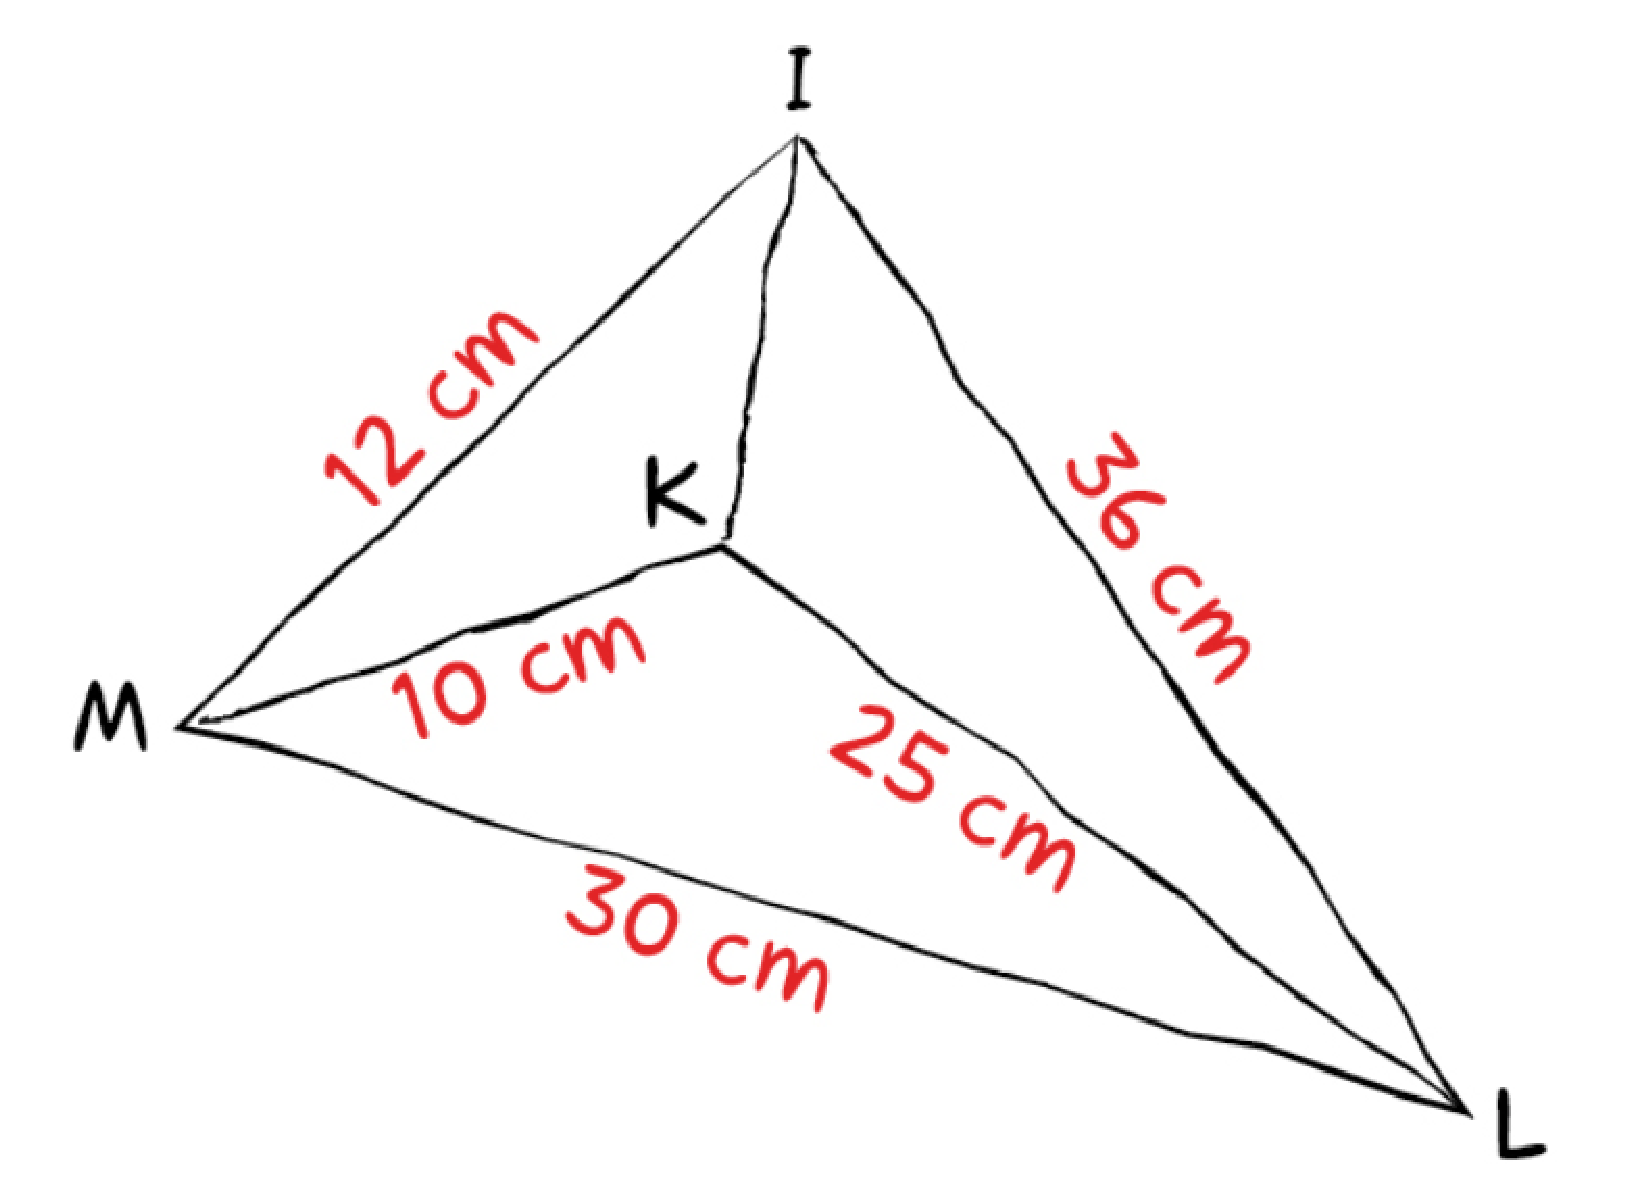
\includegraphics[scale=.18]{items/MathsP4C42.eps}

\end{center}

\end{multicols}

\end{minipage}

\vspace{0.5cm}

\medskip
\newpage
%%%%%%%%%%%%%%%%%%%%%%%%%%%%%%%%%%%%%%%%
%%%%%%%%%%%%%%%%%%%%%%%%%%%%%%%%%%%%%%%%
\setcounter{exo}{0}

%%%%%%%%%%%%%%%%%%%%%%%%%%%%%%%%%%%%%%%%
%  entête du sujet
%%%%%%%%%%%%%%%%%%%%%%%%%%%%%%%%%%%%%%%%

Collège Coat Mez de Daoulas  \hfill  le 22/01/2023

Classe : 6e A \hfill François KERMAREC

\begin{center}
\begin{LARGE} Évaluation de mathématiques \end{LARGE}
\end{center}

%\vspace*{1.5cm}




%%%%%%%%%%%%%%%%%%%%%%%%%%%%%%%%%%%%%%%
% Tableau des compétences (début)
%%%%%%%%%%%%%%%%%%%%%%%%%%%%%%%%%%%%%%%
\begin{footnotesize}

\begin{center}

\begin{tabular}{|p{120mm}|p{8mm}|p{10mm}|p{8mm}|p{8mm}|p{8mm}|}

\hline
\textbf{Compétences évaluées} & \textbf{Rouge} & \textbf{Orange} & \textbf{Bleu} & \textbf{Vert} & \textbf{Autre} \\
\hline


*  Simplifier une fraction donnée pour la rendre irréductible  & & & & & \\ 
\hline
*  Reconnaître et utiliser des triangles semblables.  & & & & & \\ 
\hline
\end{tabular}
\end{center}
\end{footnotesize}
\begin{minipage}{0.99\linewidth}

\exo

Dans cet exercice l'usage de la calculatrice est interdit.

\begin{enumerate}

\item Simplifier et rendre irréductible la fraction $\dfrac{360}{450}$ (méthode libre, mais il faut détailler les calculs).
\item Décomposer $54$ en produit de facteurs premiers.
\item Décomposer $210$ en produit de facteurs premiers.
\item Utiliser les résultats des deux questions précédentes pour rendre irréductible la fraction $\dfrac{54}{210}$
\end{enumerate}
\end{minipage}

\vspace{0.5cm}

\medskip
\begin{minipage}{0.99\linewidth}

\exo

Dans le triangle $BGF$, on sait que $\widehat{FBG}$ mesure $46$\degre et que $\widehat{BGF}$ mesure $103$\degre. On sait aussi que D est un point du segment $[BF]$, que C est un point du segment $[BG]$ et que $\widehat{BDC}$ mesure $31$\degre.

		\begin{enumerate}
		\item Faire un croquis, sur la copie, et y coder les informations données.
		\item Prouver que les triangles $BCD$ et $BFG$ sont semblables.
		\item $BD= 4$~cm, $DC=3$~cm et $BF=6$~cm. Quel est le coefficient d'agrandissement qui permet de passer du triangle $BCD$ au triangle $BFG$ ? (Justifier votre réponse).
		\end{enumerate}	

\end{minipage}

\vspace{0.5cm}
\medskip
\newpage
\end{document}
